\documentclass[]{scrartcl}
\title{Vorlesung Analysis II}
\usepackage{amsmath,amssymb,amsfonts}
\usepackage{stmaryrd}
\usepackage{mathtools}
\usepackage{latexsym}
\usepackage{graphicx}
\usepackage{tikz}
\usepackage{xcolor}
\usepackage[most]{tcolorbox}
\usepackage{soul}
\usepackage{ upgreek }
\usepackage{hyperref}
\usepackage{tipa}
\usepackage[dvipsnames]{xcolor}
\hypersetup{
	colorlinks=true,
	linkcolor=blue,
	filecolor=magenta,      
	urlcolor=cyan,
	pdftitle={Overleaf Example},
	pdfpagemode=FullScreen,
}
\newcommand{\redcircle}[1]{%
	\tikz[baseline=(char.base)]{
		\node[shape=circle, draw=red, text=red, thick, inner sep=1pt] (char) 
		{\textbf{#1}};
	}%
}
\newcommand{\bluecircle}[1]{%
	\tikz[baseline=(char.base)]{
		\node[shape=circle, draw=blue, text=blue, thick, inner sep=1pt] (char) 
		{\textbf{#1}};
	}%
}
\newcommand{\blackcircle}[1]{%
	\tikz[baseline=(char.base)]{
		\node[shape=circle, draw=black, text=black, thick, inner sep=1pt] 
		(char) 
		{\textbf{#1}};
	}%
}
\newcommand{\orangecircle}[1]{%
	\tikz[baseline=(char.base)]{
		\node[shape=circle, draw=orange, text=orange, thick, inner sep=1pt] 
		(char) 
		{\textbf{#1}};
	}%
}
\newcommand{\redul}[1]{\setulcolor{red}{\ul{#1}}}
\newcommand{\blueul}[1]{\setulcolor{blue}{\ul{#1}}}
\newcommand{\yelul}[1]{\setulcolor{yellow}{\ul{#1}}}
\newcommand{\greenul}[1]{\setulcolor{green}{\ul{#1}}}
\newcommand{\oraul}[1]{\setulcolor{orange}{\ul{#1}}}
\setul{1pt}{3pt} % Linienhöhe und Abstand zum Text (optional anpassbar)

\setlength{\topmargin}{-.5in} \setlength{\textheight}{9.25in}
\setlength{\oddsidemargin}{0in} \setlength{\textwidth}{6.8in}
\setlength{\parindent}{0pt}

\begin{document}
	\textbf{\underline{Teil 3: Gewöhnliche Differentialgleichungen}}\\
	\\
	\textbf{\underline{an16: Differentialgleichungen ind Richtungsfelder}}\\
	\\
	\textbf{\underline{\underline{Stichworte:} DGL, gewöhnliche DGL, Lösungsfunktion, Fragestellungen, Richtungsfelder}}\\
	\\
	\textbf{\underline{Literatur:}}\blueul{[Hoffmann], Kapitel 7.1}\\
	\\
	\textbf{16.1. \underline{Einleitung:}} Wir geben die Definition einer Differentialgleichung als Funktionalglg. zwischen gesuchten Fkt. y=y(x), der VAriablen x und Ableitungen con y.\\
	\\
	\textbf{16.2. \underline{Motivation:}} Gleichungen mit einer Funktion y und ihrer Ableitungen y',y'',... nennt man \redul{Differentialgleichungen}, Wir möchten solche nach y "auflösen", also Methoden zum Auffinden der Lösungsfunktion für y erarbeiten. Darin soll y in nur einer rellen Variablen x erklärt sein. Wir schreiben kurz \yelul{GDL} für "differentialgleichung".\\
	\\
	\textbf{16.3. \underline{Def.:}} Sei $k\in\mathbb{N}, \o \neq D\subseteq \mathbb{R} \times \mathbb{C}^{k+1}, F:D\rightarrow\mathbb{C}.$\\
	Dann heißt eine Glg. der Form\\
	\blackcircle{*} \yelul{$F(x,y,y',y'',...,y^{(k)})=0$}\\
	eine \redul{gewöhnliche Differentialgleichung}. (Identifiziere $\mathbb{C}$ mit $\mathbb{R}^2$)
	\\
	\textbf{16.4. \underline{Gesucht:}} ein $IV j\subseteq \mathbb{R}, y:j \rightarrow \mathbb{C}$ k-mal diff'bar\\
	mit: $\forall x \in j:	(x,y(x), y'(x),...,y^{(k)}(x))\in D$\\
	und $\forall x \in f:$ \blackcircle{*}\\
	\\
	\textbf{16.5. \underline{Bez.:}} (1) y heißt dann eine \redul{Lösung} von \blackcircle{*} (in j), Kurz: \redul{Lsg.}.\\
	man sagt, y "erfüllt die" DGL oder "genügt der" DGL.\\
	(2) Kann \blackcircle{*} speziell ind der Form $y^{k}= \phi(x,y,y',...,y^{k-1})$ geschrieben werden, dann heißt die DGL \redul{explizit},\\
	und k heißt die \redul{Ordnung} der DGL.\\
	\\
	\textbf{16.6. \underline{Bsp.:}} y'=10y ist explizit von 1. Ordnung, eine Lsg$\neq$ 0 ist $y(x)=163e^{10x}$.\\
	\\
	\textbf{16.7. \underline{Fragen:}}\\
	1. Existiert eine Lsg.? Existiert eine "lokale" Lsg.?\\
	2. Falls ja: Wie gewinnt man eine Lsg.?\\
	3. Falls ja: Eindeutigkeit?(mehrere Lösungen)\\
	4. Maximale Lsg? (bzgl. Fortsetzung der Def. menge j)\\
	5. Abhängigkeit der Lsgn. von Parametern?\\
	6. Charakterisierung der Lsgn.?\\
	\\
	\underline{Zu 1./2.:} Bsp unlösbare DGL: $(y')^2+1=0$\\
	Bsp. lösbare DGL: $y'=\phi(x)\Rightarrow y(x)=\int^{x}\phi(x)dx$ Stammfkt. von $\phi$, nicht immer leicht!\\
	\underline{Zu 3.:} Eindeutigkeit ist i.a. sinnvoll bei Vorgabe von Anfangswerten, man spricht von \redul{Anfangswerteaufgaben} \yelul{(AWA)},\\
	Auch: von Anfangswertproblemen (AWP).\\
	$\bullet$\underline{y'=10y} kann unter Vorgabe von y(0)=163 eindeutig gelöst werden, diese ist dann $y(x)=163e^{10x}$.\\
	$\bullet$ \underline{Bsp.:} $y'=\sqrt{y} (y\geq 0)$ hat unter Vorgabe von y(0)=0(lokal)unendlich viele Lsgn., vgl. Bsp. \blueul{17.10.}\\
	\\
	Man zeigt weitreichende \redul{Existenz- und Eindeutigkeitssätze}, etwa den \redul{Existenz- und Eindeutigkeitssatz von Picard-Lindelöf} (davon gibt es eine globale und eine lokale Version).\\
	\\
	\underline{Zu 4.:} Die Aufgabenstellung fragt nicht nach "Größe" von j. Interessant sind Lösungen auf möglichst große Intervall j.\\
	\underline{Bsp.:} $y'=y^2, y(0)c\textgreater0$, hier kann die Existenz nur "lokal" gesucht werden, vgl. Bsp. \blueul{17.12.}\\
	\underline{Zu 5.:} Die Abhängigkeit der Lösungen von Eingabedaten ist relevant.\\
	\underline{Zu 6.:} Man sucht nach strukturellen Eigenshaften  der Lösungsmenge.\\
	Veranschaulichungen durch \redul{Richtungsfelder} (für explizite DGL 1. Ordnung):\\
	\\
	\underline{Vereinbarung:} Betr. die DGL \blackcircle{*}\fcolorbox{red}{white}{$y'\phi(x,y)$}.\\
	\underline{Interpretation:} $\phi$ ordner jedem Punkt $(x,y)\in D$, wo $\phi:D\rightarrow \mathbb{R}$, eine Steigung/Richtung zu.\\
	\underline{Graphisch:} Zeichne in (x,y) ein kleines Geradenstück dieser Richtung ein ("\redul{Linienelemente}")\\
	Das Ergebnis im Koordinatensystem ist ein Richungsfeld.\\
	$\rightarrow$ Kurven, die in jedem (x,y) das dortige (vorgegebene) Linienelement als Tangent haben, entsprechen Lösungen der DGL.\\
	\\
	\underline{Bsp.:} $y'=y-x^2$, Bild s. \blueul{[Hoffmann, S. 236 in §7.1]}\\
	\begin{figure}[h]
		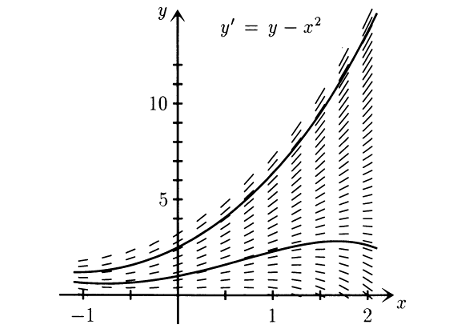
\includegraphics[width=9 cm,height=6cm]{bsp kap 16.7.1}
	\end{figure}\\ 
	\\
	\underline{Bsp.:} $y'=\frac{1}{2}y$  (die r.S. $\phi$ hängt nur von y ab)
	\begin{figure}[h]
		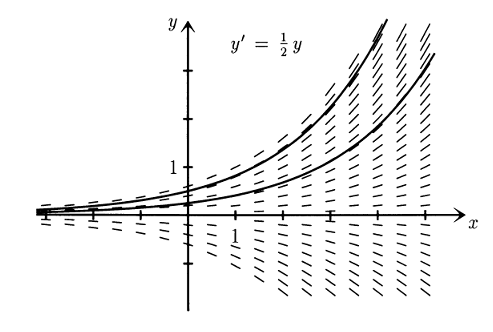
\includegraphics[width=9 cm,height=6cm]{bsp kap 16.7.2}
	\end{figure}\\ 
	\\
	\underline{Bsp:} $y'=-\frac{x}{y}, y(a)=b \textgreater0$, hat als Lösung \underline{Halbkreise} $y(x)=\sqrt{r^2-k^2}, -r\textless x\textless r,$ wo $r=\sqrt{a^2+b^2}$.\\
	\begin{figure}[h]
		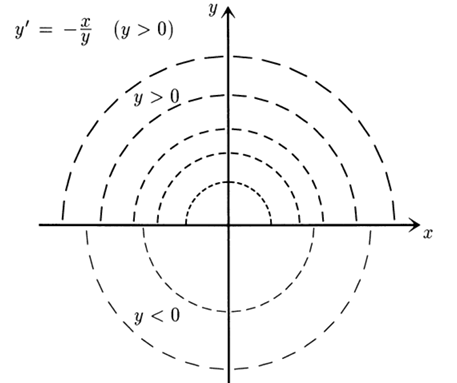
\includegraphics[width=8 cm,height=6cm]{bsp kap 16.7.3}
	\end{figure}\\ 
	\underline{Bsp.:} $y'=\frac{x}{y}, x\textgreater 0, y(a)=b$, wo $a\textgreater0,$ hat als Lösung \underline{Halbgeraden} $y(x)=\frac{b}{a}x, x\textgreater0.$\\
	\begin{figure}[h]
		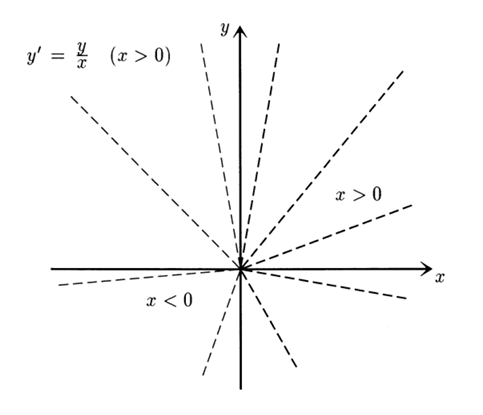
\includegraphics[width=8 cm,height=6cm]{bsp kap 16.7.4}
	\end{figure}\\ 
	
	
	
	
	
	
	
	
	
\end{document}